\section{Oversikt over verktøy}

Det er en egen kunst å finne relevante stillinger, enten det gjelder internships, deltidsjobber eller faste stillinger. I dette avsnittet vil jeg introdusere noen nyttige verktøy for prosessen, og hvordan du bruker de riktige søkeordene på ulike plattformer. Nøkkelen ligger i å optimalisere søkene dine, og etter mye prøving og feiling har jeg kommet frem til noen konklusjoner som jeg vil dele i de påfølgende avsnittene.

\begin{figure}[H]
    \centering
    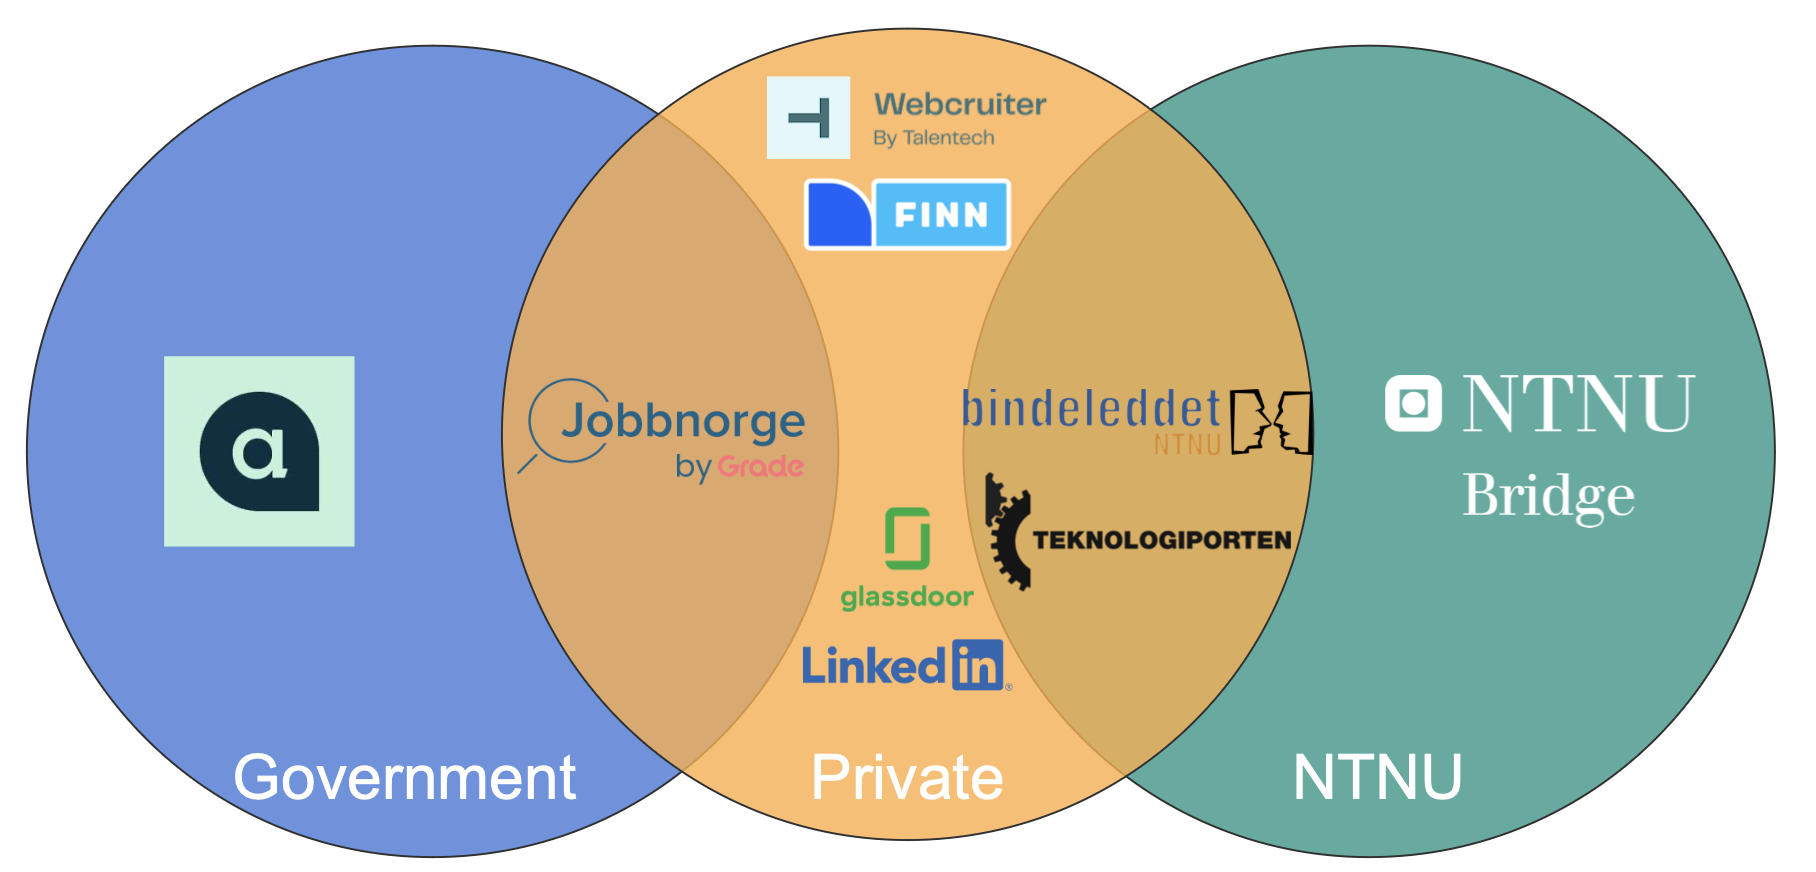
\includegraphics[width=0.8\linewidth]{images/Venn-diagram.png}
\end{figure}



\section{Finn.no}

Dette er uten tvil Norges største jobbplattform, men det handler om å bruke det smart. Inne på Finn kan man opprette nøkkelord slik at du får en varsel når jobbannonser tilknyttet disse kommer ut. Det finnes mange måter gjøre det på, men her er nøkkelordene som jeg liker å bruke:

\begin{itemize}
    \item summer intern 
    \item summer internship
    \item sommerjobb ingeniør 
    \item sommerjobb teknisk
\end{itemize}

\begin{itemize}
    \item graduate 202X
    \item nyutdannet 202X
    \item sivilingeniør
\end{itemize}

Det jeg vil anbefale er å begynne å scrolle tidlig. Jeg hadde tilfeldigvis lagret annonser fra fjoråret og da kan man se endringen fra i fjor til i år, noe som gir verdifull informasjon. Når man har lagret en annonse så er den fortsatt tilgjengelig på Finn for alle med lenken, og dette er gull verdt! Jeg har et Excel-ark som inneholder alle relevante annonser og hvis man lagrer Finn-lenken så har man likevel tilgang selv etter at det har blitt deaktivert. 


\section{LinkedIn}

LinkedIn kan beskrives som corporate versjonen av Facebook, hvor folk av og til legger ut litt kleine innlegg (og ja, jeg snakker også om meg selv). Fun fact: LinkedIn er eid av Microsoft. Av en eller annen grunn synes jeg det er utrolig gøy å klikke inn på profiler for å se hva folk driver med. Men LinkedIn er ikke bare til for nettverking – det er også en utmerket plattform for å finne jobber, noe LinkedIn tjener penger på. Akkurat som på Finn.no kan du opprette nøkkelord og sette opp varsler for stillinger som passer dine interesser. Det som skiller LinkedIn er at det er en internasjonal plattform, og større selskaper foretrekker ofte å poste stillingsannonser der fremfor på Finn.no – kanskje fordi det er billigere, men hvem vet?

\begin{remark}
    \textbf{PROTIP STALKING} Når man klikker inn på profiler på LinkedIn får vedkommende varsel om at du har vært der inne, det er kleint. Det du derimot kan gjøre er å gå inn på LinkedIn sine innstillinger og skru det av. Dette kan du ofte gjøre ved å klikke på <<Meg>>-ikonet øverst på LinkedIn-siden og deretter velge <<Innstillinger \& Personvern>> fra nedtrekksmenyen. I innstillinger og personvern, finn og klikk på <<Personvern>>-fanen som finnes langs toppen eller på siden av skjermen. Gå til <<Profilvisningsalternativer>>. Scroll ned til du finner en seksjon relatert til hvordan andre ser din aktivitet og profil, for eksempel <<Profilvisning i privatmodus>>.
\end{remark}


\section{Glassdoor}

Denne plattformen er relativt ukjent og prøver på flere måter å etterligne LinkedIn. Den brukes primært til å legge igjen anmeldelser av arbeidsgivere samt til å dele lønnsstatistikk. Informasjonen du finner der kan variere, men jeg kan dele en personlig erfaring hvor jeg hadde fått et intervju og bestemte meg for å kikke litt rundt på plattformen. Der fant jeg noen intervjuspørsmål som andre hadde delt fra samme selskap. Jeg tenkte over spørsmålet, men håpet at det ikke ville dukke opp på intervjuet – noe det selvsagt gjorde (akkurat som på en eksamen). Heldigvis var jeg forberedt siden jeg hadde vært innom Glassdoor, og den delen av intervjuet gikk bra (jeg røk dessverre ut av andre årsaker).


\section{NTNU-plattformer}

Det mange ikke vet er at det finnes en rekke plattformer som spesifikt etterspør NTNU-studenter. Disse er som følger: 

\begin{enumerate}
    \item NTNU Bridge
    \item Bindeleddet
    \item Teknologiporten
    \item HC Bedriftsider
\end{enumerate}

Jeg syntes ofte at det kan dukke opp artige stillinger på Bridge og Bindeleddet som man ellers ikke finner så kikk gjerne der også. 


\section{Karrieredager}

Det arrangeres svært mange karrieredager rundt omkring på Gløs. Her er det en liste over mange av dem og når på året det arrangeres. 

\begin{table}[H]
    \centering
    \begin{tabular}{p{2cm}p{3cm}p{7cm}}
        \toprule
        Navn & Tid & Beskrivelse \\
        \midrule
         Karrieredagene & 4 dager, starten av september & Arrangeres av Bindeleddet/indøk. Den største karrieredagen og tidlig på året. Reklameres for som om det er for hele NTNU, mens de stikker av med pengene. I 2023 var det inntekt på 3.3 mill. \cite{underdusken_tjora_karrieredagen}. \\
         IT-dagene & 2 dager, september & Arrangeres av data og komtek. \\
         Maskin- og Energidagen & 1 dag, september & Arrangeres av Maskin- og energiteknologi eller Produktutvikling og Produksjon. \\
         Kjemidagen & 1 dag, slutten av oktober & Arrangeres av nano og MTKJ. \\
         Bedriftsdagen & 1 dag, oktober & Arrangeres av marin. \\
         Energidagen & 1 dag, oktober & Arrangere av EMIL. \\
         Materialdagen & 1 dag, oktober & Arrangeres av MTMT \\
         Workation & 1 dag, okt-nov & Arrangeres av Workation, interesseorganisasjon for sommerjobb i Trondheim \\
         BM-dagen & 1 dag, starten av november & Arrangeres av bygg og miljø, inntjening på 1.8 mill. om jeg ikke har regnet feil \cite{bm_dagen_2023}. \\
         Eureka & 1 dag, januar & Arrangeres av FysMat \\
         Nettverksdagene & 3 dager, januar & Arrangeres av Kyb \\
         IV-dagene & 3 dager, februar & Av alle Ingeniørvitenskap og IKT \\
         Prospective & 2 dager, februar & Arrangeres av Teknologiporten \\
         RevolveDagen & 1 dag, februar & Arrangeres av studentorganisasjonen RevolveNTNU \\
         IAESTEs Næringslivsdager & 1 dag, mars & Av IAESTE \\
        \bottomrule
    \end{tabular}
    \caption{Oversikt over noen utvalgte karrieredager}
    \label{tab:Casekonkurranser}
\end{table}

Komplett liste finner du også på Bridge \cite{ntnu_bridge_career_days}.




\section{Svarteliste}

Denne delen er nok kontroversiell, men jeg vil påpeke at ikke alle selskaper opptrer profesjonelle til enhver tid. Det finnes mindre eksempler som det bildet under, men også noen verre eksempler jeg ønsker å påpeke.

\begin{figure}[H]
    \centering
    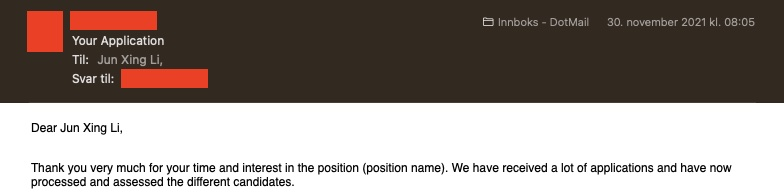
\includegraphics[width=1\linewidth]{images/mail.jpg}
\end{figure}

De verre eksemplene er mer rettet mot IT-studenter, men kan være relevant for noen fra MTKJ. Det har seg slik at noen konsulentselskaper har terminert kontrakten til sommerstudenter helt plutselig, eller permittert dem. Dette er noe som skjer i industrien under økonomisk tyngre perioder, men det er viktig å håndtere dette riktig.

\begin{figure}[H]
    \centering
    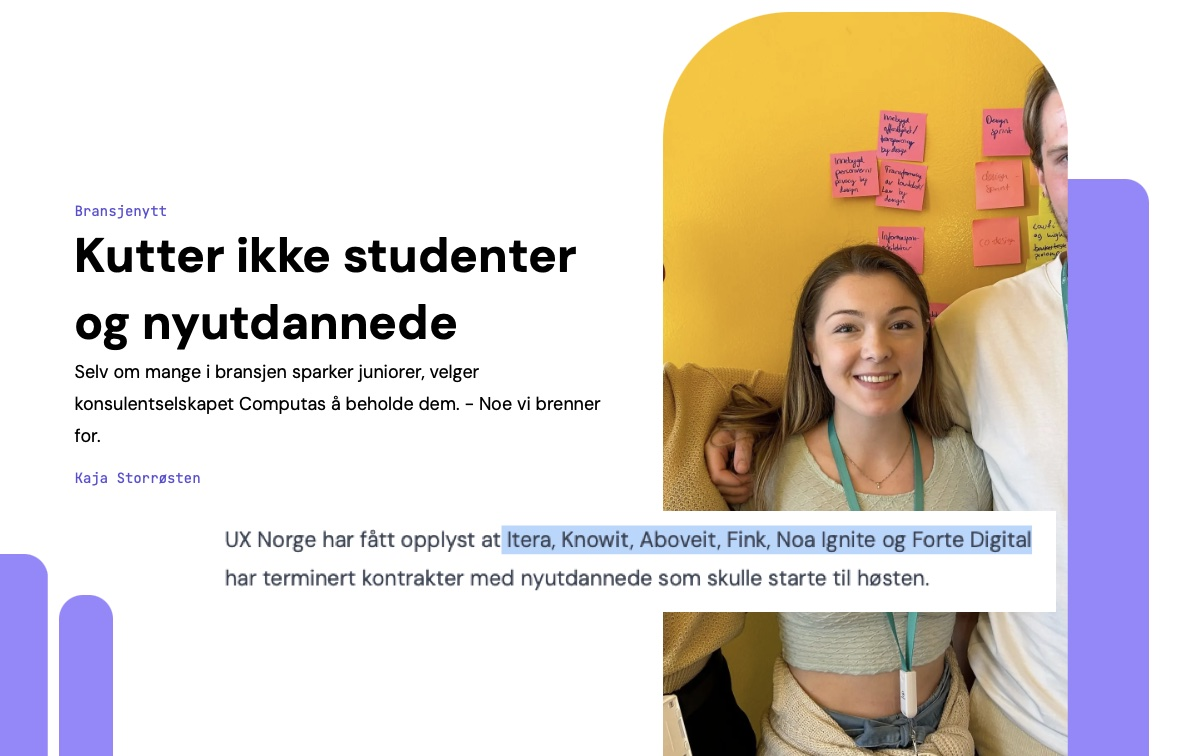
\includegraphics[width=0.8\linewidth]{images/uxnorge.jpg}
    \caption{Eksempel på hvilke selskaper som kuttet folk \cite{UXNorge2023}.}
\end{figure}